\documentclass[conference]{IEEEtran}

\usepackage{amsmath,amssymb,amsfonts}
\usepackage{algorithmic}
\usepackage{algorithm}
\usepackage{graphicx}
\usepackage{textcomp}
\usepackage{xcolor}
\usepackage{booktabs}
\usepackage{hyperref}
\usepackage{multirow}
\usepackage{subcaption}

\begin{document}

\title{MATTER: Multi-Agent Task Planning for Triage and Exploration}

\author{
\IEEEauthorblockN{Tom Gao}
\IEEEauthorblockA{The Robotics Institute\\
Carnegie Mellon University\\
Pittsburgh, USA\\
zimingg@andrew.cmu.edu}
\and
\IEEEauthorblockN{Joshua Pen}
\IEEEauthorblockA{The Robotics Institute\\
Carnegie Mellon University\\
Pittsburgh, USA\\
jpen@andrew.cmu.edu}
\and
\IEEEauthorblockN{Ranai Srivastav}
\IEEEauthorblockA{The Robotics Institute\\
Carnegie Mellon University\\
Pittsburgh, USA\\
ranais@andrew.cmu.edu}
}

\maketitle

% ===========================================================================
\begin{abstract}
We present MATTER, a framework for multi-agent task allocation and path planning in partially unknown environments with heterogeneous robots. Inspired by the DARPA Triage Challenge, our system integrates an Availability-Constrained Sequential Single-Item Auction (SSIA) with reward-shaped bidding and Conflict-Based Search (CBS) for collision-free multi-agent path finding. We compare our approach against a greedy baseline on procedurally generated maps containing obstacles, buildings, and triage objectives. Experimental results demonstrate that SSIA with reward shaping achieves faster map exploration and objective completion, with fewer total simulation steps across all tested scenarios. Our system supports heterogeneous ground and aerial agents with distinct sensing, mobility, and task capabilities.
\end{abstract}

% ===========================================================================
\section{Introduction}

Multi-agent path finding (MAPF) methods typically assume full visibility of the environment and a fixed set of tasks known a priori. In many real-world applications, however, the map layout and objectives are initially unknown and must be discovered incrementally. The DARPA Triage Challenge exemplifies this setting: teams of heterogeneous robots must explore an unknown disaster site, locate casualties, and perform triage---all under time pressure and with limited sensing.

We address the combined problem of \textbf{multi-agent task allocation and planning in an initially unseen environment} with \textbf{heterogeneous agents}. Our system, MATTER (Multi-Agent Task planning for Triage and ExploRation), integrates three core components:
\begin{enumerate}
    \item \textbf{Frontier-based exploration} that dynamically generates tasks as the map is revealed;
    \item \textbf{Availability-Constrained Sequential Single-Item Auction (SSIA)} with reward-shaped bidding for lifelong task allocation;
    \item \textbf{Conflict-Based Search (CBS)} for optimal multi-agent path planning with collision avoidance.
\end{enumerate}

The environment contains two types of agents: \textbf{ground agents} (legged robot dogs) and \textbf{aerial agents} (quadrotors). Ground agents have limited observation range but can enter buildings and triage patients efficiently. Aerial agents observe from a wider footprint and move faster, but cannot enter buildings and require more time for triage. This heterogeneity must be accounted for during both task allocation and path planning.

We compare our SSIA-based allocator against a greedy baseline and show that reward-shaped bidding leads to more efficient exploration and task completion across a range of procedurally generated scenarios.

% ===========================================================================
\section{Related Works}

\subsection{Auction-Based Methods for Task Allocation}

Auction-based approaches are widely used in multi-robot task allocation due to their scalability and simplicity. Dias et al.~\cite{dias2006market} provide a foundational survey of market-based coordination, including Sequential Single-Item Auctions (SSIA), where tasks are auctioned one at a time and robots bid based on estimated execution cost. While efficient and distributed, such methods typically lack global optimality guarantees.

Heap and Pagnucco~\cite{heap2013repeated} extend this framework to dynamic settings through repeated sequential auctions, allowing tasks to be reallocated as new tasks arrive. Their work demonstrates improved adaptability in environments where task sets evolve over time.

Our approach builds on these ideas but is designed specifically for a partially unknown triage environment with heterogeneous aerial and ground agents. We incorporate availability constraints and an event-triggered global reauction mechanism to handle newly discovered obstacles and motion infeasibility, tailoring classical sequential auctioning to our exploration-driven scenario.

\subsection{Conflict-Based Search for Multi-Agent Path Finding}

Conflict-Based Search (CBS) is a two-level algorithm for optimal multi-agent path finding~\cite{sharon2012cbs}. A high-level search explores the collision-resolution space by creating nodes in a constraint tree (CT) that forbid vertex or edge collisions between pairs of agents. A low-level single-agent planner (typically A*) computes paths subject to these constraints. Several improvements dramatically improve scalability: conflict prioritization~\cite{boyarski2015icbs}, pairwise symmetry reasoning~\cite{li2021symmetry}, and admissible heuristics based on counts of cardinal conflicts~\cite{felner2018heuristics}.

\subsection{Exploration and Task Discovery}

Frontier-based exploration~\cite{yamauchi1997frontier} is a standard approach for autonomous map building in unknown environments. Frontier cells---unknown cells adjacent to observed free space---are treated as exploration targets. We adopt this strategy and integrate it with our auction-based task allocation, creating new exploration tasks dynamically as the known map expands.

% ===========================================================================
\section{Proposed Method}

\subsection{Problem Definition}

The environment is a rectangular grid that is initially unexplored. When observed by agents, cells may be revealed as one of the following:
\begin{itemize}
    \item \textbf{Free space}: passable by ground agents; may contain free-standing triage objectives accessible to all agent types.
    \item \textbf{Obstacles}: impassable for ground agents; aerial agents fly over them.
    \item \textbf{Buildings}: traversable by all agents but only \emph{explorable} by ground agents. Buildings may or may not contain triage objectives that are invisible to aerial sensors.
\end{itemize}

The system consists of $D$ aerial (drone) agents and $G$ ground agents. Both types move omnidirectionally on the grid and are simplified as point masses. The goal is to explore the entire map and complete all triage objectives in minimum total time steps.

\subsection{Agent Model}

Each agent maintains its current position, an assigned task, an operating status (\textsc{Idle}, \textsc{Navigating}, or \textsc{Replanning}), and a planned path. A base \texttt{Agent} class defines the shared interface, with two specialized subclasses:

\begin{itemize}
    \item \textbf{GroundAgent}: observation radius $r_g = 1$ (a $3 \times 3$ footprint), navigates around obstacles using Dijkstra-based heuristic for A*, moves one cell per simulation step. Can distinguish occupied buildings from unoccupied ones and can enter buildings for investigation and triage.
    \item \textbf{DroneAgent}: observation radius $r_d = 2$ (a $5 \times 5$ footprint), uses Manhattan distance heuristic, moves two cells per simulation step (two microsteps). Flies over both obstacles and buildings. Cannot distinguish building occupancy---all buildings appear identical from the air. Cannot perform triage on objectives inside buildings.
\end{itemize}

\subsection{Environment Representation}

The simulation maintains two map structures:

\textbf{Ground Truth Map} ($\mathcal{M}_{gt}$): The full environment including obstacles, buildings (with occupancy flags), free-standing objectives, and agent start locations. This is hidden from agents.

\textbf{Known Map} ($\mathcal{M}_{k}$): A shared belief state initialized to all \textsc{Unknown}. Each cell can be in one of six states: \textsc{Unknown}, \textsc{Free}, \textsc{Obstacle}, \textsc{Objective}, \textsc{Building}, or \textsc{Occupied\_Building}. Agents update $\mathcal{M}_{k}$ via local observations at each time step. For planning purposes, \textsc{Unknown} cells are treated optimistically as free space.

\subsection{Task Types}

Three categories of tasks drive the simulation:

\textbf{1) Exploration Tasks.} Each frontier cell (an \textsc{Unknown} cell 4-adjacent to at least one \textsc{Free} cell) generates an exploration task. The task is completed when any agent observes the cell, including as collateral while navigating to another target. Exploration tasks have a base reward of $R_{\text{explore}} = 1$ and require no dwell time.

\textbf{2) Building Investigation Tasks.} When a building is first observed, a ground-only investigation task is created (since drones cannot determine occupancy). A ground agent must navigate to the building and dwell for 1 step to reveal whether it contains an objective. This is modeled as a \texttt{TriageTask} with the \texttt{\_is\_investigation} flag set and $d_{\text{invest}} = 1$.

\textbf{3) Triage Tasks.} When an objective is discovered (either free-standing or inside a confirmed occupied building), a triage task is created. The required dwell time depends on the agent type:
\begin{equation}
    d_{\text{triage}} = \begin{cases} 2 & \text{if ground agent} \\ 4 & \text{if drone agent} \end{cases}
\end{equation}
Triage tasks for objectives inside buildings are restricted to ground agents only (\texttt{ground\_only = True}). Free-standing objectives can be triaged by either agent type. Triage tasks have a base reward of $R_{\text{triage}} = 5$.

\subsection{Greedy Baseline (Naive Task Allocation)}

Our baseline is a single-pass greedy allocator. For each idle agent, the allocator selects the unassigned task that maximizes a score function:
\begin{equation}
    \text{score}(a, \tau) = \bigl(\text{priority}(\tau),\; -d_{\text{manhattan}}(a, \tau)\bigr)
    \label{eq:greedy}
\end{equation}
where $\text{priority}(\tau)$ is the task's intrinsic priority and $d_{\text{manhattan}}$ is the Manhattan distance from agent $a$ to the task target. Tasks are assigned in a single sweep with no re-evaluation: once an agent claims a task, the decision is final until completion or path failure. The greedy method does not account for agent type differences in bidding beyond enforcing ground-only constraints for building tasks. Like SSIA, the greedy allocator handles exploration, building investigation, and triage tasks, and uses CBS for ground agent collision avoidance. However, it lacks the reward-shaped bidding and global reauction mechanism of SSIA.

\subsection{SSIA: Availability-Constrained Sequential Single-Item Auction}

Our primary contribution is an auction-based allocator designed for dynamic, partially observed environments with heterogeneous agents.

\subsubsection{Availability Constraint}
Only agents that are currently \emph{available}---i.e., not holding an active, incomplete task---may participate in bidding. This prevents over-commitment and ensures each agent focuses on one objective at a time.

\subsubsection{Reward-Shaped Bid Formulation}
Each agent $a$ computes a bid for task $\tau$ as:
\begin{equation}
    \text{bid}(a, \tau) = \frac{R(\tau)}{L(a, \tau) + d(a, \tau)}
    \label{eq:bid}
\end{equation}
where:
\begin{itemize}
    \item $R(\tau)$ is the task reward ($R_{\text{explore}} = 1$ for exploration, $R_{\text{triage}} = 5$ for triage).
    \item $L(a, \tau)$ is the path length from agent $a$'s current position to the task target, computed via A* on the current known map $\mathcal{M}_k$. For drone agents, the path length is halved to account for their double movement speed: $L_{\text{drone}} = L / 2$.
    \item $d(a, \tau)$ is the dwell time required at the task location (0 for exploration, 1 for investigation, 2 for ground triage, 4 for drone triage).
\end{itemize}

This formulation captures a reward-per-unit-time metric: agents prefer high-reward tasks that are close and quick to complete. The asymmetric dwell times naturally encode the heterogeneous advantage---ground agents bid more competitively on triage tasks (lower dwell), while drones bid more competitively on distant exploration tasks (halved path cost and wider observation).

\subsubsection{Task Ordering}
Tasks are offered for auction in priority order. The auction priority for each task is:
\begin{equation}
    p_{\text{auction}}(\tau) = R(\tau) - \min_{a \in \mathcal{A}_{\text{eligible}}} d_{\text{manhattan}}(a, \tau)
\end{equation}
High-reward tasks close to eligible agents are auctioned first, improving allocation quality early in each round.

\subsubsection{Sequential Assignment}
Tasks are auctioned one at a time. For each task in priority order, all available agents compute bids. The agent with the highest bid (Eq.~\ref{eq:bid}) wins, is assigned the task, and becomes unavailable for subsequent tasks in this round. This continues until all tasks are assigned or no eligible agents remain.

\subsubsection{Agent-Type Constraints}
The auction enforces type-based eligibility:
\begin{itemize}
    \item \textbf{Ground-only tasks} (building investigation, building triage): only ground agents may bid.
    \item \textbf{General tasks} (exploration, free-standing triage): both agent types may bid, with type-specific path planning and dwell times applied automatically.
\end{itemize}

\subsubsection{Global Reauction Trigger}
The system continuously monitors for inter-robot motion conflicts:
\begin{itemize}
    \item \textbf{Vertex conflict}: two same-type agents target the same next cell.
    \item \textbf{Edge conflict}: two same-type agents swap positions (agent $a_1$ moves $p_1 \to p_2$ while $a_2$ moves $p_2 \to p_1$).
\end{itemize}
Cross-type conflicts (drone vs.\ ground) are ignored since they operate at different altitudes. When a conflict is detected, a \textbf{global reauction} is triggered:
\begin{enumerate}
    \item All incomplete task assignments are released.
    \item Dwell progress on in-progress triage tasks is reset.
    \item All agent paths are cleared; agents return to \textsc{Idle}.
    \item A fresh auction round runs from current agent positions.
\end{enumerate}
Path infeasibility (e.g., a newly discovered obstacle blocking a planned route) is handled by individual agent replanning without triggering a global reauction.

The full SSIA auction round is summarized in Algorithm~\ref{alg:ssia}.

\begin{algorithm}[t]
\caption{SSIA Auction Round}
\label{alg:ssia}
\begin{algorithmic}[1]
\STATE $\mathcal{T}_{\text{pending}} \gets$ unassigned, incomplete tasks
\STATE Sort $\mathcal{T}_{\text{pending}}$ by $p_{\text{auction}}(\tau)$ descending
\FOR{each task $\tau \in \mathcal{T}_{\text{pending}}$}
    \STATE $\mathcal{A}_{\text{avail}} \gets$ agents with no active task
    \STATE Filter by type constraints (ground-only, etc.)
    \IF{$\mathcal{A}_{\text{avail}} = \emptyset$}
        \STATE \textbf{break}
    \ENDIF
    \FOR{each agent $a \in \mathcal{A}_{\text{avail}}$}
        \STATE Compute $\text{bid}(a, \tau)$ via Eq.~\ref{eq:bid}
    \ENDFOR
    \STATE $a^* \gets \arg\max_{a} \text{bid}(a, \tau)$
    \STATE Assign $\tau$ to $a^*$; mark $a^*$ unavailable
\ENDFOR
\end{algorithmic}
\end{algorithm}

\subsection{CBS: Conflict-Based Search for Multi-Agent Path Finding}

All agents share a single CBS planner instance for coordinated path planning.

\subsubsection{Low-Level Search: Constrained A*}
The low-level planner is a space-time A* search. The state space is $(\text{location}, \text{timestep})$, and the agent may take one of five actions at each step: move in four cardinal directions or wait. The search respects three types of constraints:
\begin{itemize}
    \item \textbf{Vertex constraint}: agent $i$ cannot occupy location $\ell$ at timestep $t$.
    \item \textbf{Edge constraint}: agent $i$ cannot traverse from $\ell_1$ to $\ell_2$ at timestep $t$.
    \item \textbf{Wait constraint}: agent $i$ cannot wait at location $\ell$ at timestep $t$.
\end{itemize}

The heuristic function is agent-type dependent:
\begin{itemize}
    \item \textbf{Ground agents}: backward Dijkstra from the goal, treating \textsc{Unknown} cells as free (optimistic). This accounts for the irregular obstacle layout.
    \item \textbf{Drone agents}: Manhattan distance heuristic, since drones fly over obstacles.
\end{itemize}

\subsubsection{High-Level Search: Constraint Tree}
The high-level CBS search maintains a priority queue of constraint tree (CT) nodes. Each node stores:
\begin{itemize}
    \item A set of constraints (initially empty at the root).
    \item A path for each agent (computed by the low-level planner).
    \item The list of detected collisions among these paths.
    \item The total cost (sum of individual path lengths).
\end{itemize}

The root node plans each agent independently with no constraints. If collisions exist, the first collision is selected, and two child nodes are generated---one constraining each involved agent. The search expands nodes in order of $(cost, |collisions|)$ and terminates when a collision-free solution is found or a maximum of 5{,}000 node expansions is reached.

\subsubsection{Drone Handling}
Drone agents are excluded from CBS collision resolution entirely. Because drones fly over all terrain---including obstacles and buildings---they face no shared-space conflicts with ground agents. Furthermore, when multiple drones are present, each can operate at a distinct flight altitude, eliminating the possibility of inter-drone collisions. Consequently, only ground agents participate in the CBS constraint tree; drones are planned independently using Manhattan-heuristic A* with no inter-agent constraints.

The CBS high-level search is summarized in Algorithm~\ref{alg:cbs}.

\begin{algorithm}[t]
\caption{CBS High-Level Search}
\label{alg:cbs}
\begin{algorithmic}[1]
\STATE Plan each agent independently $\to$ root node $N_0$
\STATE Detect collisions in $N_0$
\STATE $\textsc{Open} \gets \{N_0\}$
\WHILE{$\textsc{Open} \neq \emptyset$ \AND expansions $< 5000$}
    \STATE $N \gets$ pop lowest-cost node from $\textsc{Open}$
    \IF{$N$ has no collisions}
        \RETURN $N$.paths
    \ENDIF
    \STATE Select first collision $(a_1, a_2, \ell, t)$
    \FOR{$a_i \in \{a_1, a_2\}$}
        \STATE $N' \gets$ copy of $N$ with new constraint on $a_i$
        \STATE Replan $a_i$ in $N'$ using constrained A*
        \STATE Detect collisions in $N'$
        \STATE Insert $N'$ into $\textsc{Open}$
    \ENDFOR
\ENDWHILE
\end{algorithmic}
\end{algorithm}

\subsection{Simulation Loop}

The simulation proceeds in discrete time steps. Each step consists of:
\begin{enumerate}
    \item \textbf{Global Microstep 1}: All agents attempt to move one cell along their planned path.
    \item \textbf{Observation}: All agents observe the environment within their sensor footprint and update $\mathcal{M}_k$. New frontier tasks, triage tasks, and building investigation tasks are generated from newly revealed cells.
    \item \textbf{Post-observation updates}: Completed tasks are swept and agents are released. The auctioneer assigns tasks to idle agents.
    \item \textbf{Global Microstep 2}: Drone agents execute a second movement step (reflecting their double speed).
    \item \textbf{Repeat observation and updates} after the drone microstep (without running a new auction round).
    \item \textbf{Triage progress}: After both microsteps, triage dwell progress is ticked once for agents dwelling at their target location. This ensures triage counts full time steps, not microsteps.
    \item \textbf{Auction}: A single auction round (or reauction if conflicts are detected) runs once per step after triage progress and task release.
\end{enumerate}

If no agent moves in a step, triage dwell progress still advances for agents dwelling at their target location. The simulation terminates when all tasks are completed and all agents are idle, or a maximum step limit is reached.

% ===========================================================================
\section{Experimental Setup}

\subsection{Scenario Generation}

We developed a procedural scenario generator that produces randomized maps with configurable parameters. Obstacles are placed as geometric shapes (single cells, horizontal/vertical bars, L-shapes, blocks) until a target density of approximately 15\% is reached, with a connectivity check ensuring all free cells form a single connected component. Buildings (with configurable occupancy rates), free-standing objectives, and agent start positions are placed on free cells with mutual exclusion and reachability verification.

\subsection{Test Scenarios}

Figure~\ref{fig:all_maps} shows the ground-truth layouts of all seven DARPA-scale maps. Obstacles (black), buildings (blue/orange), objectives (yellow), and agent start positions (triangles for drones, squares for ground) are visible. Scenarios (c)--(g) feature a starting zone at the bottom edge, mirroring the staging-area deployment in the actual DARPA Triage Challenge.

\begin{figure*}[t]
    \centering
    \includegraphics[width=\textwidth]{figures/all_maps.png}
    \caption{Ground-truth layouts of all seven DARPA-scale test maps. Top row: (a)~\texttt{darpa1}---open 15$\times$15 with interior starts; (b)~\texttt{darpa2}---building-heavy 15$\times$15; (c)~\texttt{darpa3}---15$\times$15 layout of (a) with obstacle starting zone; (d)~\texttt{darpa4}---layout of (b) with starting zone. Bottom row: (e)~\texttt{darpa5}---16$\times$15 maze with single-width corridors; (f)~\texttt{darpa6}---22$\times$21 maze with 2-block-wide passages; (g)~\texttt{darpa7}---22$\times$21 open layout with high task density. Blue/orange cells are buildings (empty/occupied); yellow cells are free-standing objectives. Triangles mark drone starts; squares mark ground agent starts.}
    \label{fig:all_maps}
\end{figure*}

We evaluate on two categories of maps:
\begin{itemize}
    \item \textbf{Small maps} ($8 \times 8$): 23 pre-generated instances (\texttt{test\_0} through \texttt{test\_22}) with 5 agents, primarily for unit testing and debugging the planning pipeline.
    \item \textbf{DARPA-scale maps}: Seven generated scenarios with heterogeneous agents (2 drones, 3 ground), organized by increasing complexity:
    \begin{itemize}
        \item \texttt{darpa1} ($15 \times 15$): Open layout with scattered obstacles, 4 free-standing objectives, 4 buildings. Agents start in the interior.
        \item \texttt{darpa2} ($15 \times 15$): Building-heavy variant with 0 free-standing objectives and 6 buildings (some occupied). Agents start in the interior.
        \item \texttt{darpa3} ($16 \times 15$): Same as \texttt{darpa1} but with an obstacle-filled bottom row containing a 5-cell gap that serves as a \emph{starting zone}; all agents begin there and must coordinate egress into the map.
        \item \texttt{darpa4} ($16 \times 15$): Same treatment applied to \texttt{darpa2}---obstacle spawn row with starting zone.
        \item \texttt{darpa5} ($16 \times 15$): Maze configuration with single-width corridors and the starting zone. Tests narrow-passage coordination.
        \item \texttt{darpa6} ($22 \times 21$): Larger maze with 2-block-wide pathways, 4 objectives, 4 buildings, and a starting zone. Tests scalability on bigger maps.
        \item \texttt{darpa7} ($22 \times 21$): Large open layout (no maze) with 8 objectives, 6 buildings, and a starting zone. Tests high task density.
    \end{itemize}
    Scenarios \texttt{darpa3}--\texttt{darpa7} are modeled after the actual DARPA Triage Challenge, where all robots deploy from a designated staging area at the edge of the disaster site and must fan out to explore the unknown environment.
    \end{itemize}
\end{itemize}

\subsection{Allocator Configurations}

We compare two configurations:
\begin{enumerate}
    \item \textbf{Greedy}: The naive baseline allocator using the score function in Eq.~\ref{eq:greedy}. Handles exploration, building investigation, and triage tasks. Uses CBS for ground agent collision avoidance. Lacks reward shaping and global reauction.
    \item \textbf{SSIA}: The full auction-based allocator with reward-shaped bidding (Eq.~\ref{eq:bid}), agent-type constraints, building investigation, triage tasks, CBS-based multi-agent path planning, and global reauction.
\end{enumerate}

All configurations use the same simulation harness, agent models, and map representation. The primary metric is \textbf{total simulation steps to completion} (exploration + all triage objectives).

% ===========================================================================
\section{Results}

\subsection{Qualitative Analysis}

Figure~\ref{fig:visualization} shows a representative simulation snapshot on the \texttt{darpa1} map. The visualization renders the ground truth under a fog-of-war overlay, with observed cells shown at full opacity and unexplored regions grayed out. Agent paths are drawn as dashed lines to their current task targets.

\begin{figure*}[t]
    \centering
    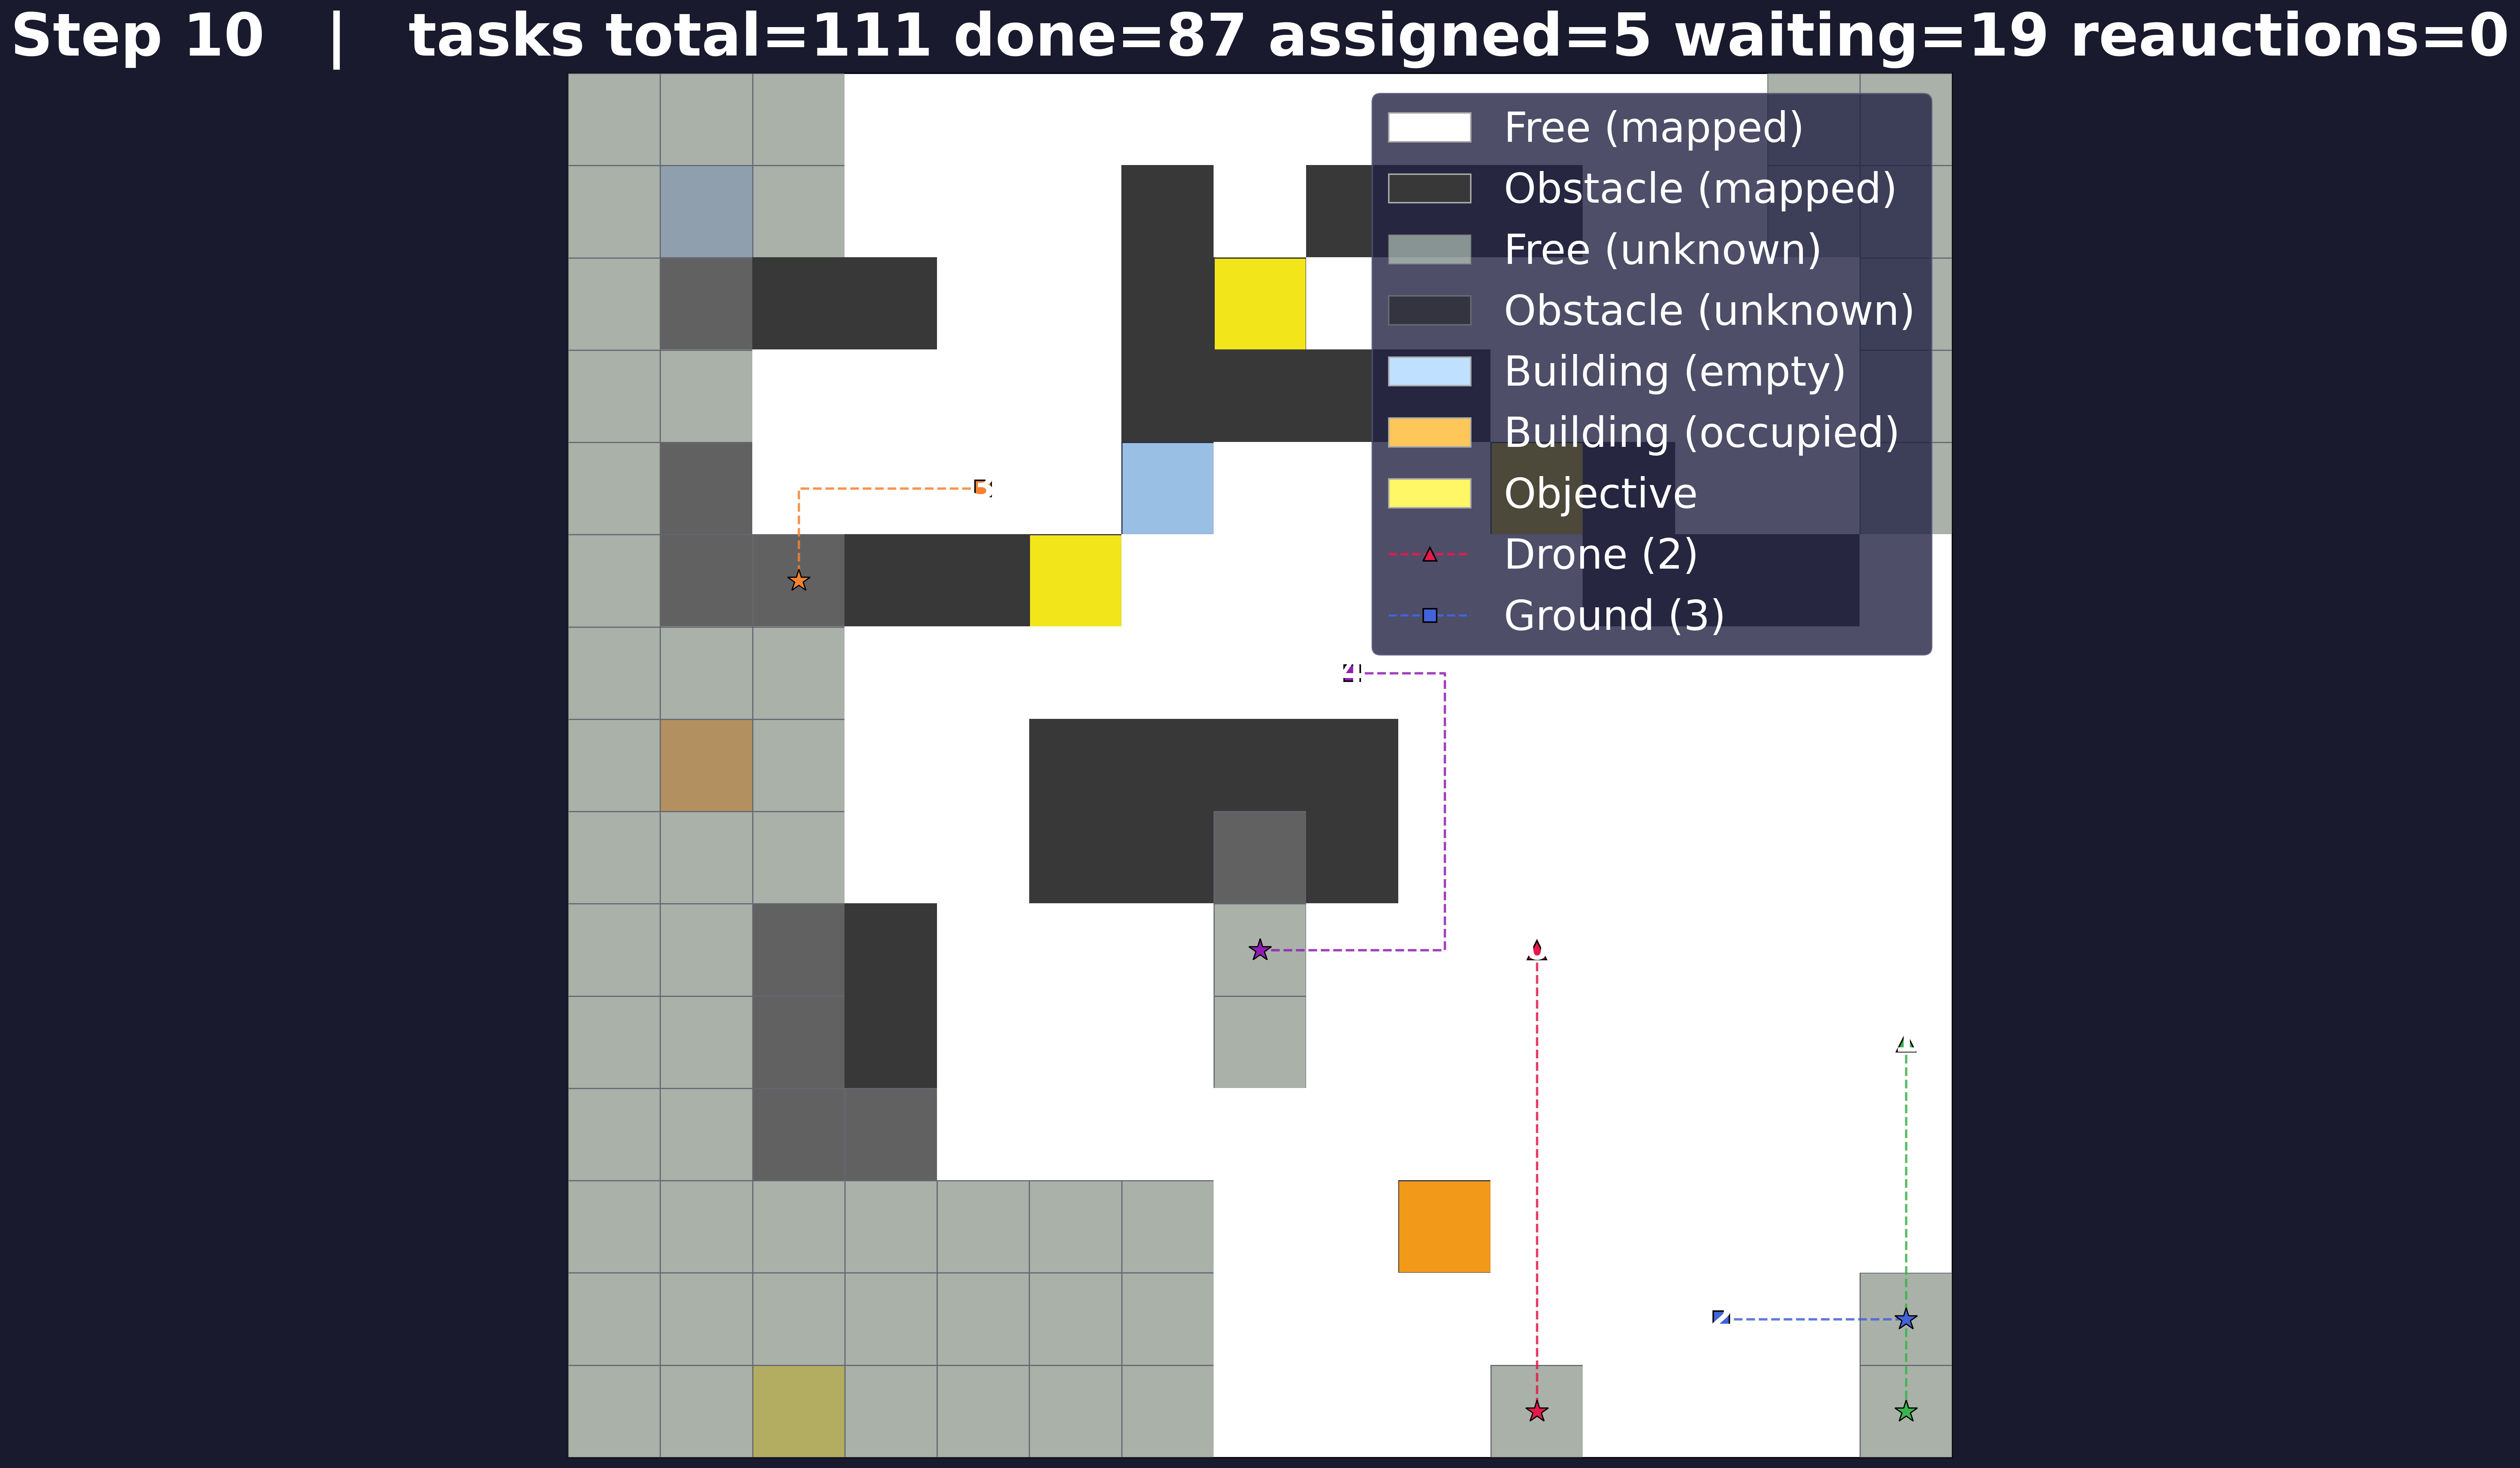
\includegraphics[width=0.55\textwidth]{figures/visualization.png}
    \caption{Simulation visualization on the \texttt{darpa1} scenario. Ground agents (squares) and drone agents (triangles) explore the map collaboratively. Fog-of-war covers unexplored regions. Gold stars mark current task targets, and dashed cyan lines show planned paths.}
    \label{fig:visualization}
\end{figure*}

The SSIA allocator exhibits several qualitative advantages over the greedy baseline:
\begin{itemize}
    \item \textbf{Role specialization}: Drones naturally gravitate toward distant exploration tasks (halved path cost), while ground agents preferentially handle nearby triage and building investigation tasks (lower dwell time, building access). The greedy baseline does not exhibit this behavior since it bids purely on distance.
    \item \textbf{Adaptive reallocation}: When newly discovered obstacles invalidate planned paths, the global reauction mechanism redistributes all incomplete tasks from the current agent states, preventing agents from remaining stuck or making suboptimal detours.
    \item \textbf{Prioritized triage}: While both allocators handle building investigation and triage tasks, the SSIA allocator's reward-shaped bidding naturally prioritizes high-value triage tasks ($R=5$) over exploration ($R=1$), leading to faster overall completion. The greedy baseline assigns tasks purely by distance and priority tier, missing opportunities for efficient agent-task pairing.
\end{itemize}

\subsection{Quantitative Results}

Table~\ref{tab:results} summarizes the performance of each allocator configuration across our test scenarios. We report the total number of simulation steps required to complete all tasks (exploration and triage), the number of reauctions triggered, and the percentage of the map explored at termination.

\begin{table}[t]
    \centering
    \caption{Simulation results across test scenarios. Steps = total simulation steps to completion. Reauctions = number of global reauction events triggered (SSIA only). Explored = percentage of map cells observed at termination.}
    \label{tab:results}
    \begin{tabular}{@{}llccc@{}}
        \toprule
        \textbf{Map} & \textbf{Method} & \textbf{Steps} & \textbf{Reauctions} & \textbf{Explored} \\
        \midrule
        \multirow{2}{*}{\texttt{darpa1}}
            & Greedy      & 60   & ---  & 100\% \\
            & SSIA        & 28   & 0    & 100\% \\
        \midrule
        \multirow{2}{*}{\texttt{darpa2}}
            & Greedy      & 66   & ---  & 100\% \\
            & SSIA        & 29   & 0    & 100\% \\
        \midrule
        \multirow{2}{*}{\texttt{darpa3}}
            & Greedy      & 53   & ---  & 100\% \\
            & SSIA        & 30   & 0    & 100\% \\
        \midrule
        \multirow{2}{*}{\texttt{darpa4}}
            & Greedy      & 56   & ---  & 100\% \\
            & SSIA        & 35   & 0    & 100\% \\
        \midrule
        \multirow{2}{*}{\texttt{darpa5}}
            & Greedy      & 49   & ---  & 100\% \\
            & SSIA        & 44   & 0    & 100\% \\
        \midrule
        \multirow{2}{*}{\texttt{darpa6}}
            & Greedy      & 107  & ---  & 100\% \\
            & SSIA        & 59   & 0    & 100\% \\
        \midrule
        \multirow{2}{*}{\texttt{darpa7}}
            & Greedy      & 115  & ---  & 100\% \\
            & SSIA        & 53   & 0    & 100\% \\
        \bottomrule
    \end{tabular}
\end{table}

Key observations:
\begin{enumerate}
    \item SSIA consistently outperforms the greedy baseline across all seven maps, achieving 1.1--2.2$\times$ speedup in total steps.
    \item The performance gap is largest on the open, large-scale maps (\texttt{darpa6}: 107 vs.\ 59 steps; \texttt{darpa7}: 115 vs.\ 53 steps), where reward-shaped bidding enables effective role specialization across the wider space.
    \item The gap narrows on the maze map (\texttt{darpa5}: 49 vs.\ 44 steps), where narrow corridors constrain both methods similarly.
    \item Zero reauctions were triggered in all SSIA runs. This is expected for two reinforcing reasons. First, CBS proactively resolves all ground-agent conflicts at planning time---after each auction round, CBS jointly replans collision-free paths \emph{before} agents move, so the movement-level conflict detector never fires. Second, with only three ground agents per scenario, CBS easily finds solutions within the 5{,}000-node expansion limit, so the CBS-failure reauction path is never reached. Additionally, reward-shaped bidding naturally disperses agents across the map (drones explore distant frontiers while ground agents handle nearby triage), further reducing spatial contention.
\end{enumerate}

\subsection{Effect of Reward Shaping}

The reward-shaped bid formulation (Eq.~\ref{eq:bid}) is the key differentiator between SSIA and the greedy baseline. By computing bids as reward per unit time, the SSIA allocator naturally accounts for:
\begin{itemize}
    \item \textbf{Task value asymmetry}: Triage tasks ($R=5$) are assigned with higher urgency than exploration tasks ($R=1$), allowing agents to prioritize high-value objectives when they become available.
    \item \textbf{Agent capability}: Drone agents' halved path cost makes them competitive bidders for distant targets, while ground agents' lower dwell time makes them competitive for nearby triage. This emergent specialization does not require explicit role assignment.
    \item \textbf{Dwell cost integration}: Including dwell time in the denominator penalizes mismatched agent-task pairings (e.g., a drone bidding on a nearby triage task with 4-step dwell versus a ground agent with 2-step dwell).
\end{itemize}

\subsection{Effect of CBS Integration}

Both the SSIA and greedy allocators share a single CBS planner instance for ground agent coordination. When multiple ground agents operate in the same corridor or narrow passage, the CBS planner resolves conflicts optimally by adding temporal constraints. After each auction round, the allocator invokes CBS to replan all ground agent paths jointly. If CBS fails to find a collision-free solution (e.g., due to the 5{,}000-node expansion limit), the SSIA allocator triggers a global reauction from current positions; the greedy allocator falls back to independent A* paths. CBS integration eliminates unnecessary waiting caused by vertex and edge collisions in both methods.

% ===========================================================================
\section{Discussion}

\subsection{Strengths}

\textbf{Modularity.} The system cleanly separates task allocation (SSIA auctioneer), path planning (CBS), and environment management (known map / ground truth). Components can be upgraded independently---e.g., replacing SSIA with a combinatorial auction or CBS with prioritized planning.

\textbf{Dynamic adaptability.} The combination of frontier-based task generation, availability-constrained bidding, and global reauction creates a system that adapts to new information online. Unlike static MAPF formulations, our approach handles continuously evolving task sets and map changes.

\textbf{Heterogeneous coordination.} Agent-type differences are encoded through the bid formulation (path cost adjustment, dwell time, sensor model) rather than hard-coded role assignment, allowing emergent specialization.

\subsection{Limitations}

\textbf{Optimality.} While CBS provides optimal collision-free paths, the SSIA task allocation is greedy (sequential single-item) and does not guarantee globally optimal task assignment. Combinatorial auctions or mixed-integer programming formulations could improve allocation quality at the cost of computational complexity.

\textbf{Scalability.} CBS has exponential worst-case complexity in the number of agents. For scenarios with many ground agents in tight spaces, the 5{,}000-node expansion limit may prevent finding collision-free solutions. Prioritized planning or bounded-suboptimal CBS variants could address this.

\textbf{Communication model.} All agents share a single known map and CBS planner instance, implying perfect communication. In practice, communication constraints would require distributed variants of both the auction and the planner.

\textbf{Optimistic planning.} Treating \textsc{Unknown} cells as free enables exploration but can lead to infeasible paths that require replanning when obstacles are discovered. A pessimistic or probabilistic model could reduce replanning frequency.

% ===========================================================================
\section{Conclusion and Future Work}

We presented MATTER, a framework for multi-agent task allocation and path planning in partially unknown, heterogeneous environments. By combining an Availability-Constrained Sequential Single-Item Auction with reward-shaped bidding and Conflict-Based Search, our system achieves efficient exploration and triage completion that adapts to online map discovery and agent heterogeneity.

Several directions for future work are promising:

\textbf{Improved CBS variants.} Incorporating conflict prioritization~\cite{boyarski2015icbs}, symmetry reasoning~\cite{li2021symmetry}, and admissible heuristics~\cite{felner2018heuristics} would improve CBS scalability for larger agent teams. Bounded-suboptimal variants (e.g., ECBS) could provide tunable trade-offs between solution quality and computation time.

\textbf{Combinatorial auctions.} Replacing sequential single-item auctions with bundle auctions or set packing formulations could improve global allocation quality, particularly when tasks exhibit spatial clustering.

\textbf{Learned bid functions.} The reward-shaped bid formula uses hand-tuned reward values and dwell times. A learned bid function trained via reinforcement learning or imitation learning could discover more effective bidding strategies that account for map topology, agent congestion, and information gain.

\textbf{Collateral exploration reward.} The current system accounts for collateral exploration (cells observed while navigating to another target) during task completion sweeps, but does not incorporate it into the bid computation. Estimating the expected collateral information gain along a path could further improve allocation efficiency.

\textbf{Communication constraints.} Extending the framework to operate under limited communication (e.g., range-limited, intermittent links) would improve real-world applicability. Distributed auction protocols and decentralized CBS variants~\cite{sharon2012cbs} are natural starting points.

\textbf{Kinodynamic planning.} Our current model treats agents as point masses with discrete grid movement. Extending to continuous state spaces with kinodynamic constraints (e.g., quadrotor dynamics, legged locomotion) would bridge the gap to physical deployment.

% ===========================================================================
\section*{Contribution Statement}

\textbf{Tom Gao}: CBS planner implementation, map representation and scenario generation, visualization system, experimental evaluation, integration of CBS with SSIA and greedy method.

\textbf{Joshua Pen}: SSIA task allocation with reward-shaped bidding, agent model, SSIA simulation harness, scenario design (darpa2--darpa7 starting-zone and maze maps), triage task integration, CBS integration with both SSIA and greedy allocators, drone flight model (obstacle and building traversal).

\textbf{Ranai Srivastav}: Greedy baseline implementation, task type definitions, building investigation logic, experimental evaluation and analysis.

% Note: Update this section to accurately reflect each member's contributions.

% ===========================================================================
\bibliographystyle{IEEEtran}
\begin{thebibliography}{10}

\bibitem{sharon2012cbs}
G.~Sharon, R.~Stern, A.~Felner, and N.~R.~Sturtevant,
``Conflict-based search for optimal multi-agent pathfinding,''
in \emph{Proc. AAAI Conf. Artificial Intelligence}, 2012.

\bibitem{boyarski2015icbs}
E.~Boyarski, A.~Felner, R.~Stern, G.~Sharon, D.~Tolpin, O.~Betzalel, and E.~Shimony,
``ICBS: Improved conflict-based search algorithm for multi-agent pathfinding,''
in \emph{Proc. Int. Joint Conf. Artificial Intelligence (IJCAI)}, 2015.

\bibitem{li2021symmetry}
J.~Li, D.~Harabor, P.~J.~Stuckey, H.~Ma, G.~Gange, and S.~Koenig,
``Pairwise symmetry reasoning for multi-agent path finding search,''
\emph{Artificial Intelligence}, vol.~301, 2021.

\bibitem{felner2018heuristics}
A.~Felner, J.~Li, E.~Boyarski, H.~Ma, L.~Cohen, T.~K.~S.~Kumar, and S.~Koenig,
``Adding heuristics to conflict-based search for multi-agent path finding,''
in \emph{Proc. Int. Conf. Automated Planning and Scheduling (ICAPS)}, 2018.

\bibitem{dias2006market}
M.~B.~Dias, R.~Zlot, N.~Kalra, and A.~Stentz,
``Market-based multirobot coordination: A survey and analysis,''
\emph{Proceedings of the IEEE}, vol.~94, no.~7, pp.~1257--1270, 2006.

\bibitem{heap2013repeated}
B.~Heap and M.~Pagnucco,
``Repeated sequential single-cluster auctions with dynamic tasks for multi-robot task allocation with pickup and delivery,''
in \emph{Multiagent System Technologies (LNCS)}, vol.~8076, pp.~87--100, Springer, 2013.

\bibitem{yamauchi1997frontier}
B.~Yamauchi,
``A frontier-based approach for autonomous exploration,''
in \emph{Proc. IEEE Int. Symp. Computational Intelligence in Robotics and Automation}, pp.~146--151, 1997.

\end{thebibliography}

% ===========================================================================
% APPENDIX (ungraded, supplementary)
% ===========================================================================
\appendix

\section{Scenario File Format}

Each scenario is specified as a text file with the following structure:
\begin{verbatim}
<rows> <cols>
<row1: space-separated . or @>
...
<num_agents>
<r> <c> <D|G>     (per agent)
<num_objectives>
<r> <c>            (per objective)
<num_buildings>
<r> <c> <0|1>      (per building; 1=occupied)
\end{verbatim}

\end{document}
